\chapter{Marginal tools}

In the course of development, I spent countless hours to experiment with ideas and methods. Many of these implementations have continued their life as the program's components. But some could not survive, regardless of how much effort I put on them. A notable one is the tool called \emph{Tokenizer}, my mini version of Lucene.

Available in \textsc{Pāli\,Platform\,2}, Tokenizer allows any number of documents to be indexed on the fly. Then this temporary collection can be searched and term-listed. In \textsc{Pāli\,Platform\,3}, I have changed the strategy by using Lucene in full range. That made Tokenizer obsolete and no longer needed. One aspect of Tokenizer that has been lost in the new implementation is the ability to include any number of documents (in Lucene Finder, text groups in indexing process are predefined, not arbitrary).

Other than Tokenizer, there are some tools that fall into the similar status but still in use. I call these tools \emph{marginal} in the sense that they may not be very useful and they are likely to be removed in the future to reduce the maintaining cost.\footnote{If someone clearly insists some need for such a tool, it may be kept and maintained. The Myanmar script conversion is one of the case. It was nearly removed but some still need it (no matter how ugly it will be).} I will talk about these in the following sections.

\section{Batch Script Transformer}

In my plan, this tool facilitates script conversion of a bunch of files. It works fine with some limitations. However, even I myself hardly use this tool substantially. When I need to convert a text collection into a new script, I normally write a new and simpler program for the task, mainly with JavaScript.

Batch Script Transformer can be launched by menu File > {\faSix \symbol{"F085}} Batch Script Transformer. Its window is shown in Figure \ref{fig:batch-script-transformer}. The functions and limitations of the tool are described as follows:

\begin{figure}[!hbt]
\centering
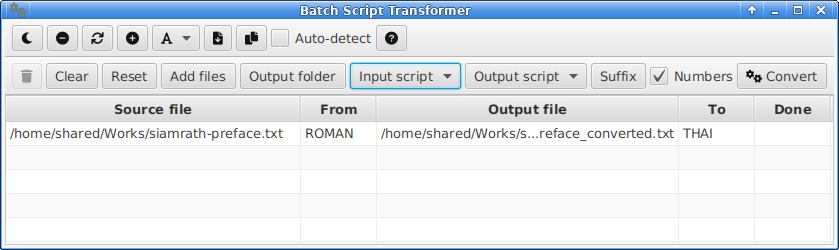
\includegraphics[width=0.9\linewidth]{images/batch-script-transformer.png}\\
\caption{Window of Batch Script Transformer}
\label{fig:batch-script-transformer}
\end{figure}

\begin{compactitem}
\item The input texts should be in plain text, not structured like XML or JSON, because the tool cannot differentiate the data from its structure. However, it can be safer to convert structured non-Roman texts into Roman script.
\item The conversion can be done from Roman source to Devanagari, Khmer, Myanmar, Sinhala, and Thai script; and from Devanagari, Khmer, Sinhala, and Thai to Roman script.
\item The input script can be auto-detected or manually specified.
\item Every transforming algorithm (except Roman to Myanmar) used here is the same as applied in the program's text viewers.
\item Devanagari conversion uses least contamination method (see Section \ref{sect:cst-xml} on page \pageref{sect:cst-xml}), targeting the CST4 documents bundled with the program.
\item Roman to Myanmar conversion (no Myanmar to Roman) uses straight conversion (not like in the program's viewers). This can produce the result comparable to that of CST4.1 program (hopefully). However, Myanmar conversion is very fragile. So, do not take the result seriously.
\item For other options and operations, please read on the internal help of the tool.
\end{compactitem}

